\documentclass{article}
%%%%%%%%%%%%%%%%%%%%%%%%%%%%%%%%%%%%%%%%%%%%%%%%%%%%%%%%%%%%%%%%%%%%%%%%%%%%%%%%
% This LaTeX document is a comprehensive study guide for a chemistry exam.
% It is structured to provide a clear, phased study plan and detailed explanations
% of practice problems relevant to the exam topics.
%
% Preamble: Loading necessary packages for formatting and functionality.
%%%%%%%%%%%%%%%%%%%%%%%%%%%%%%%%%%%%%%%%%%%%%%%%%%%%%%%%%%%%%%%%%%%%%%%%%%%%%%%%

\usepackage[letterpaper, margin=1in, textwidth=6.5in, top=0.75in, bottom=0.75in]{geometry} % Manages page layout (margins, paper size).
\usepackage{graphicx}       % Required for including images.
\usepackage{amsmath}        % Provides advanced environments for equations (like align*).
\usepackage{amssymb}        % Provides additional mathematical symbols.
\usepackage{amsfonts}       % Provides mathematical fonts.
\usepackage[shortlabels]{enumitem} % Allows for customization of list environments (e.g., adding space between items).
\usepackage{pdfpages}       % Allows for the inclusion of entire pages from external PDF files.
\usepackage{chemformula}    % Simplifies writing chemical formulas (e.g., \ch{H2O}). Very useful for chemistry documents.
\usepackage{siunitx}        % Provides standardized formatting for numbers and units (e.g., \SI{1.00}{g/mol}).
\usepackage{hyperref}       % Creates hyperlinks within the document, useful for navigation in PDF viewers.
\usepackage{xcolor}         % Provides color capabilities.
\usepackage{sectsty}        % Allows customization of section headings.
\usepackage{lipsum}         % For generating placeholder text (not used in final version, but good for testing).

% Customizing section headings to make them stand out.
\allsectionsfont{\sffamily\bfseries\color{blue!60!black}}

% Setup for hyperlinks to be colored for better visibility.
\hypersetup{
    colorlinks=true,
    linkcolor=blue,
    filecolor=magenta,      
    urlcolor=cyan,
}

% DOCUMENT METADATA
\title{\sffamily\bfseries Comprehensive Study Guide for Chemistry Exam 2}
\author{} % Author and date are left blank as requested for a clean study guide format.
\date{}

\begin{document}

\maketitle % Generates the title.
\thispagestyle{empty} % Removes page number from the title page.

%========================================================================================
% CHAPTER 5: IONIC AND COVALENT COMPOUNDS
%========================================================================================
\section*{Chapter 5: Ionic and Covalent Compounds}

\subsection*{Ionic vs. Molecular Compounds}
\begin{itemize}[itemsep=5pt]
    \item \textbf{Ionic Compound:} A compound formed from the electrostatic attraction between a \textbf{metal cation} (positive ion) and a \textbf{nonmetal anion} (negative ion). Electrons are transferred from the metal to the nonmetal. Example: \ch{NaCl} (Sodium is a metal, Chlorine is a nonmetal).
    \item \textbf{Molecular (Covalent) Compound:} A compound formed from the sharing of electrons between two or more \textbf{nonmetals}. Example: \ch{H2O} (Hydrogen and Oxygen are both nonmetals).
\end{itemize}

\subsubsection*{Practice: Classifying Ionic Compounds}
\begin{enumerate}[itemsep=5pt]
    \item \textbf{Classify \ch{MgCl2}:} Magnesium (Mg) is a Group 2 metal. Chlorine (Cl) is a Group 17 nonmetal. This is a metal-nonmetal combination, so it is \textbf{ionic}.
    \item \textbf{Classify \ch{FePO4}:} Iron (Fe) is a transition metal. Phosphate (\ch{PO4^3-}) is a polyatomic anion. The compound consists of a metal cation and an anion, making it \textbf{ionic}.
    \item \textbf{Classify \ch{K3N}:} Potassium (K) is a Group 1 metal. Nitrogen (N) is a Group 15 nonmetal. This is a metal-nonmetal combination, so it is \textbf{ionic}.
    \item \textbf{Classify \ch{CuSO4}:} Copper (Cu) is a transition metal. Sulfate (\ch{SO4^2-}) is a polyatomic anion. The compound is formed between a metal cation and an anion, making it \textbf{ionic}.
    \item \textbf{Classify \ch{NH4Cl}:} Ammonium (\ch{NH4+}) is a polyatomic cation (composed of nonmetals). Chloride (\ch{Cl-}) is a nonmetal anion. Even though it's made entirely of nonmetals, the bond is between a cation and an anion, so it is classified as \textbf{ionic}.
\end{enumerate}

\subsubsection*{Practice: Classifying Molecular Compounds}
\begin{enumerate}[itemsep=5pt]
    \item \textbf{Classify \ch{CO2}:} Carbon (C) is a nonmetal. Oxygen (O) is a nonmetal. This is a nonmetal-nonmetal combination, so it is \textbf{molecular}.
    \item \textbf{Classify \ch{P4O10}:} Phosphorus (P) is a nonmetal. Oxygen (O) is a nonmetal. This is a nonmetal-nonmetal combination, so it is \textbf{molecular}.
    \item \textbf{Classify \ch{S2Cl4}:} Sulfur (S) is a nonmetal. Chlorine (Cl) is a nonmetal. This is a nonmetal-nonmetal combination, so it is \textbf{molecular}.
    \item \textbf{Classify \ch{NBr3}:} Nitrogen (N) is a nonmetal. Bromine (Br) is a nonmetal. This is a nonmetal-nonmetal combination, so it is \textbf{molecular}.
    \item \textbf{Classify \ch{H2S}:} Hydrogen (H) is a nonmetal. Sulfur (S) is a nonmetal. This is a nonmetal-nonmetal combination, so it is \textbf{molecular}.
\end{enumerate}

\subsection*{Lattice Energy}
\begin{itemize}[itemsep=5pt]
    \item \textbf{Definition:} Lattice energy is a measure of the stability of an ionic solid. It is the energy released when gaseous ions combine to form one mole of a solid ionic compound. A higher lattice energy indicates a stronger ionic bond and a more stable compound.
    \item \textbf{Trends:} Lattice energy is governed by Coulomb's Law: \( E \propto \frac{|Q_1 \times Q_2|}{d} \)
    \begin{itemize}
        \item \textbf{Ionic Charge (Q):} Lattice energy increases dramatically as the magnitude of the ionic charges increases. This is the most important factor.
        \item \textbf{Ionic Radius (distance, d):} Lattice energy decreases as the size of the ions increases (because the distance between their centers increases).
    \end{itemize}
\end{itemize}

\subsubsection*{Practice Problems: Ranking by Lattice Energy}
\begin{enumerate}[itemsep=5pt]
    \item \textbf{Arrange in order of increasing lattice energy: KCl, SrS, RbI.}
    \begin{itemize}
        \item \textbf{Charges:} KCl (+1,-1), SrS (+2,-2), RbI (+1,-1).
        \item \textbf{Analysis:} SrS has the highest product of charges (|+2 \(\times\) -2| = 4), so it will have the highest lattice energy. Both KCl and RbI have a charge product of 1. Between them, \ch{Rb+} is larger than \ch{K+} and \ch{I-} is larger than \ch{Cl-}. Therefore, the distance in RbI is greater, giving it a lower lattice energy than KCl.
        \item \textbf{Answer:} \textbf{RbI < KCl < SrS}
    \end{itemize}
    \item \textbf{Arrange in order of increasing lattice energy: \ch{AlF3}, \ch{AlCl3}, \ch{AlBr3}.}
    \begin{itemize}
        \item \textbf{Charges:} All compounds involve \ch{Al^3+} and a halide ion (\ch{X-}). The charge factor is the same for all.
        \item \textbf{Radius:} The size of the anions increases down the group: \ch{F-} < \ch{Cl-} < \ch{Br-}.
        \item \textbf{Conclusion:} Since lattice energy is inversely proportional to ionic radius, the compound with the smallest anion (\ch{AlF3}) will have the highest lattice energy.
        \item \textbf{Answer:} \textbf{\ch{AlBr3} < \ch{AlCl3} < \ch{AlF3}}
    \end{itemize}
    \item \textbf{Which has the higher lattice energy: NaF or MgO?}
    \begin{itemize}
        \item \textbf{Charges:} NaF has (+1, -1) ions. MgO has (+2, -2) ions.
        \item \textbf{Conclusion:} The product of charges for MgO (4) is much greater than for NaF (1). This charge difference is the dominant factor, making the lattice energy of \textbf{MgO} significantly higher.
    \end{itemize}
    \item \textbf{Arrange in order of increasing lattice energy: \ch{MgCl2}, \ch{BeCl2}, \ch{CaCl2}.}
    \begin{itemize}
        \item \textbf{Charges:} All compounds contain a Group 2 cation (+2) and chloride anions (-1). The charge factor is the same.
        \item \textbf{Radius:} The size of the cations increases down the group: \ch{Be^2+} < \ch{Mg^2+} < \ch{Ca^2+}.
        \item \textbf{Conclusion:} The compound with the smallest cation (\ch{BeCl2}) has the smallest distance between ions and thus the highest lattice energy.
        \item \textbf{Answer:} \textbf{\ch{CaCl2} < \ch{MgCl2} < \ch{BeCl2}}
    \end{itemize}
    \item \textbf{Arrange in order of increasing lattice energy: NaCl, MgS, AlP.}
    \begin{itemize}
        \item \textbf{Charges:} NaCl (+1, -1), MgS (+2, -2), AlP (+3, -3).
        \item \textbf{Conclusion:} The product of the ionic charges increases significantly (1, 4, 9). This is the dominant factor.
        \item \textbf{Answer:} \textbf{NaCl < MgS < AlP}
    \end{itemize}
\end{enumerate}

\subsection*{Predicting Ionic Formulas (Criss-Cross Method)}
\textbf{To Do:} Predict the chemical formula of an ionic compound by balancing the charges. The total positive charge from the cations must equal the total negative charge from the anions. The "criss-cross" method is a shortcut: the magnitude of the charge on one ion becomes the subscript for the other ion. Always simplify the subscripts to the smallest whole-number ratio.

\subsubsection*{Practice Problems: Predicting Formulas}
\begin{enumerate}[itemsep=5pt]
    \item \textbf{Formula for Aluminum Oxide:} Aluminum (Group 13) is \ch{Al^3+}. Oxide (Group 16) is \ch{O^2-}. Criss-crossing the charges gives \textbf{\ch{Al2O3}}.
    \item \textbf{Formula for Magnesium Nitride:} Magnesium (Group 2) is \ch{Mg^2+}. Nitride (Group 15) is \ch{N^3-}. Criss-crossing the charges gives \textbf{\ch{Mg3N2}}.
    \item \textbf{Formula for Scandium (III) Hydroxide:} Scandium (III) is \ch{Sc^3+}. Hydroxide is the polyatomic ion \ch{OH-}. Criss-crossing gives \ch{Sc(OH)3}. Parentheses are required around the polyatomic ion. The formula is \textbf{\ch{Sc(OH)3}}.
    \item \textbf{Formula for Tin (IV) Sulfate:} Tin (IV) is \ch{Sn^4+}. Sulfate is \ch{SO4^2-}. Criss-crossing gives \ch{Sn2(SO4)4}. The subscripts (2 and 4) can be simplified by dividing by 2. The final formula is \textbf{\ch{Sn(SO4)2}}.
    \item \textbf{Formula for Ammonium Phosphate:} Ammonium is \ch{NH4+}. Phosphate is \ch{PO4^3-}. Criss-crossing gives \ch{(NH4)3PO4}. The formula is \textbf{\ch{(NH4)3PO4}}.
\end{enumerate}

\subsection*{Nomenclature Practice (Mixed Types)}
\subsubsection*{Practice: Naming Compounds}
\begin{enumerate}[itemsep=5pt]
    \item \textbf{Name \ch{Fe2(SO4)3}:} Ionic. \ch{SO4} is sulfate (-2 charge). Total negative is -6. Two Fe ions must balance this, so each is \ch{Fe^3+}. Name: \textbf{Iron (III) sulfate}.
    \item \textbf{Name \ch{P2S5}:} Molecular. Two phosphorus, five sulfur. Name: \textbf{Diphosphorus pentasulfide}.
    \item \textbf{Name \ch{HBr(aq)}:} Acid. Binary acid (H + nonmetal). Rule: hydro- + (nonmetal root) + -ic acid. Name: \textbf{Hydrobromic acid}.
    \item \textbf{Name \ch{CuSO4*5H2O}:} Hydrate. Name the ionic part first: \ch{CuSO4} is Copper (II) sulfate. The prefix for 5 is "penta-". Name: \textbf{Copper (II) sulfate pentahydrate}.
    \item \textbf{Name \ch{HNO2(aq)}:} Acid. Oxoacid. The anion is \ch{NO2-} (nitrite). Rule: Anions ending in "-ite" become "-ous acid". Name: \textbf{Nitrous acid}.
\end{enumerate}

\subsubsection*{Practice: Writing Formulas from Names}
\begin{enumerate}[itemsep=5pt]
    \item \textbf{Formula for Chromium (VI) oxide:} Ionic. \ch{Cr^6+} and \ch{O^2-}. Criss-cross and simplify: \ch{Cr2O6} $\rightarrow$ \textbf{\ch{CrO3}}.
    \item \textbf{Formula for Dinitrogen trioxide:} Molecular. "di-" = 2 Nitrogen. "tri-" = 3 Oxygen. Formula: \textbf{\ch{N2O3}}.
    \item \textbf{Formula for Perchloric acid:} Oxoacid. "-ic acid" comes from an "-ate" anion. Perchlorate is \ch{ClO4-}. Balance with \ch{H+}. Formula: \textbf{\ch{HClO4}}.
    \item \textbf{Formula for Magnesium sulfate heptahydrate:} Ionic hydrate. Magnesium is \ch{Mg^2+}. Sulfate is \ch{SO4^2-}. They combine 1:1 to form \ch{MgSO4}. "hepta-" means 7 waters. Formula: \textbf{\ch{MgSO4 * 7H2O}}.
    \item \textbf{Formula for Vanadium (V) chloride:} Ionic. \ch{V^5+} and \ch{Cl-}. Criss-cross. Formula: \textbf{\ch{VCl5}}.
\end{enumerate}

\subsection*{Empirical vs. Molecular Formulas}
\subsubsection*{Practice: Deducing Empirical Formulas}
\begin{enumerate}[itemsep=5pt]
    \item \textbf{Dextrose (Molecular Formula \ch{C6H12O6}):} Divide subscripts (6, 12, 6) by their greatest common divisor (6). Empirical Formula: \textbf{\ch{CH2O}}.
    \item \textbf{Adenine (Molecular Formula \ch{C5H5N5}):} Divide subscripts (5, 5, 5) by 5. Empirical Formula: \textbf{CHN}.
    \item \textbf{Nitrous Oxide (Molecular Formula \ch{N2O}):} Subscripts (2, 1) are already in their simplest whole-number ratio. Empirical Formula: \textbf{\ch{N2O}}.
    \item \textbf{Octane (Molecular Formula \ch{C8H18}):} Divide subscripts (8, 18) by their greatest common divisor (2). Empirical Formula: \textbf{\ch{C4H9}}.
    \item \textbf{Hydrogen Peroxide (Molecular Formula \ch{H2O2}):} Divide subscripts (2, 2) by 2. Empirical Formula: \textbf{HO}.
\end{enumerate}

\subsection*{Molar Mass and Percent Composition}
\begin{itemize}[itemsep=5pt]
    \item \textbf{Molar Mass:} The mass in grams of one mole of a substance (\si{g/mol}). Calculated by summing the atomic masses of all atoms in the formula.
    \item \textbf{Percent Composition:} The percentage by mass of each element in a compound.
    \[ \text{\% mass of element} = \frac{(n \times \text{molar mass of element})}{\text{molar mass of compound}} \times 100\% \]
\end{itemize}

\subsubsection*{Practice: Molar Mass \& Percent Composition}
\begin{enumerate}[itemsep=5pt]
    \item \textbf{Calculate the molar mass of Barium Acetate, \ch{Ba(C2H3O2)2}.}
    \[ 1(\SI{137.33}{g/mol}) + 4(\SI{12.01}{g/mol}) + 6(\SI{1.008}{g/mol}) + 4(\SI{16.00}{g/mol}) = \textbf{\SI{255.42}{g/mol}} \]
    \item \textbf{Calculate the mass percent of nitrogen in ammonium nitrate (\ch{NH4NO3}).}
    \begin{itemize}
        \item \textbf{Molar Mass:} \(2(\SI{14.01}{g/mol}) + 4(\SI{1.008}{g/mol}) + 3(\SI{16.00}{g/mol}) = \SI{80.05}{g/mol}\)
        \item \textbf{Percent N:} \( \frac{2 \times \SI{14.01}{g/mol}}{\SI{80.05}{g/mol}} \times 100\% = \textbf{35.0\%} \)
    \end{itemize}
    \item \textbf{Calculate the molar mass of Ibuprofen (\ch{C13H18O2}).}
     \[ 13(\SI{12.01}{g/mol}) + 18(\SI{1.008}{g/mol}) + 2(\SI{16.00}{g/mol}) = \textbf{\SI{206.28}{g/mol}} \]
    \item \textbf{Calculate the mass percent of carbon in propane (\ch{C3H8}).}
     \begin{itemize}
        \item \textbf{Molar Mass:} \(3(\SI{12.01}{g/mol}) + 8(\SI{1.008}{g/mol}) = \SI{44.09}{g/mol}\)
        \item \textbf{Percent C:} \( \frac{3 \times \SI{12.01}{g/mol}}{\SI{44.09}{g/mol}} \times 100\% = \textbf{81.7\%} \)
    \end{itemize}
    \item \textbf{How many moles are in \SI{25.0}{g} of calcium nitrate, \ch{Ca(NO3)2}?}
     \begin{itemize}
        \item \textbf{Molar Mass:} \(40.08 + 2(14.01) + 6(16.00) = \SI{164.1}{g/mol}\)
        \item \textbf{Moles:} \( 25.0 \text{ g} \times \frac{1 \text{ mol}}{\SI{164.1}{g}} = \textbf{0.152 mol} \)
    \end{itemize}
\end{enumerate}

\section*{Chapter 8: Chemical Reactions}

\subsection*{Balancing Equations and Classifying Reactions}
\subsubsection*{Practice: Balancing and Classifying}
\begin{enumerate}[itemsep=5pt]
    \item \textbf{\_ \ch{Ca(OH)2(aq)} + \_ \ch{Al2(SO4)3(aq)} -> \_ \ch{CaSO4(s)} + \_ \ch{Al(OH)3(s)}}
    \begin{itemize}
        \item \textbf{Balance:} Balance the polyatomic ions first. There are 3 \ch{SO4} on the left, so put a 3 in front of \ch{CaSO4}. This creates 3 Ca, so put a 3 in front of \ch{Ca(OH)2}. Now there are 6 OH groups on the left, so put a 2 in front of \ch{Al(OH)3} to balance the OH and the Al.
        \item \textbf{Answer:} \textbf{\ch{3 Ca(OH)2 + Al2(SO4)3 -> 3 CaSO4 + 2 Al(OH)3}}
        \item \textbf{Classification:} Two ionic compounds swap ions. This is \textbf{Double Replacement}.
    \end{itemize}
    \item \textbf{\_ \ch{Mg(s)} + \_ \ch{Fe2O3(s)} -> \_ \ch{Fe(s)} + \_ \ch{MgO(s)}}
    \begin{itemize}
        \item \textbf{Balance:} Balance Fe first by placing a 2 in front of Fe. Balance O by placing a 3 in front of MgO. This creates 3 Mg, so place a 3 in front of Mg.
        \item \textbf{Answer:} \textbf{\ch{3 Mg(s) + Fe2O3(s) -> 2 Fe(s) + 3 MgO(s)}}
        \item \textbf{Classification:} Magnesium replaces iron in the compound. This is \textbf{Single Replacement}.
    \end{itemize}
    \item \textbf{\_ \ch{C2H4(g)} + \_ \ch{O2(g)} -> \_ \ch{CO2(g)} + \_ \ch{H2O(g)}}
    \begin{itemize}
        \item \textbf{Balance:} Balance C: 2 \ch{CO2}. Balance H: 2 \ch{H2O}. Count O on right: \(2 \times 2 + 2 \times 1 = 6\). Balance O on left: 3 \ch{O2}.
        \item \textbf{Answer:} \textbf{\ch{C2H4(g) + 3 O2(g) -> 2 CO2(g) + 2 H2O(g)}}
        \item \textbf{Classification:} Hydrocarbon reacts with oxygen. This is \textbf{Combustion}.
    \end{itemize}
    \item \textbf{\_ \ch{PbSO4(s)} -> \_ \ch{PbSO3(s)} + \_ \ch{O2(g)}}
    \begin{itemize}
        \item \textbf{Balance:} Balance Pb and S (they are 1:1). Balance O. There are 4 on left, 5 on right. Double the lead compounds to get an even number of oxygens.
        \item \textbf{Answer:} \textbf{\ch{2 PbSO4(s) -> 2 PbSO3(s) + O2(g)}}
        \item \textbf{Classification:} One compound breaks into multiple products. This is \textbf{Decomposition}.
    \end{itemize}
    \item \textbf{\_ \ch{P2O5(s)} + \_ \ch{H2O(l)} -> \_ \ch{H3PO4(aq)}}
    \begin{itemize}
        \item \textbf{Balance:} Balance P by putting a 2 in front of \ch{H3PO4}. This gives 6 H, so put a 3 in front of \ch{H2O}. Check O: 5 + 3 = 8 on left, \(2 \times 4 = 8\) on right. It is balanced.
        \item \textbf{Answer:} \textbf{\ch{P2O5(s) + 3 H2O(l) -> 2 H3PO4(aq)}}
        \item \textbf{Classification:} Two reactants form one product. This is \textbf{Synthesis (Combination)}.
    \end{itemize}
\end{enumerate}

\subsection*{Stoichiometry and Limiting Reactants}
\begin{itemize}[itemsep=5pt]
    \item \textbf{Stoichiometry:} Using the mole ratios from a balanced chemical equation to calculate the amounts of reactants consumed or products formed.
    \item \textbf{Limiting Reactant:} The reactant that is completely consumed first in a reaction, thereby limiting the amount of product that can be formed.
    \item \textbf{Theoretical Yield:} The maximum amount of product that can be produced from the given amounts of reactants, calculated based on the limiting reactant.
    \item \textbf{Percent Yield:} The ratio of the actual yield (the amount of product actually obtained) to the theoretical yield, expressed as a percentage.
\end{itemize}

\subsubsection*{Practice: Limiting Reactant, Yield, and Excess}
\begin{enumerate}[itemsep=5pt]
    \item \textbf{Problem:} Given \ch{2 Na + Br2 -> 2 NaBr}. If you have \SI{46.0}{g} of Na and \SI{150.0}{g} of \ch{Br2}, what is the theoretical yield of NaBr?
    \begin{itemize}
        \item \textbf{Molar Masses:} Na = \SI{22.99}{g/mol}, \ch{Br2} = \SI{159.8}{g/mol}, NaBr = \SI{102.89}{g/mol}.
        \item \textbf{From Na:} \( 46.0 \text{ g Na} \times \frac{1 \text{ mol Na}}{22.99 \text{ g}} \times \frac{2 \text{ mol NaBr}}{2 \text{ mol Na}} \times \frac{102.89 \text{ g NaBr}}{1 \text{ mol NaBr}} = 206 \text{ g NaBr} \)
        \item \textbf{From \ch{Br2}:} \( 150.0 \text{ g } \ch{Br2} \times \frac{1 \text{ mol } \ch{Br2}}{159.8 \text{ g}} \times \frac{2 \text{ mol NaBr}}{1 \text{ mol } \ch{Br2}} \times \frac{102.89 \text{ g NaBr}}{1 \text{ mol NaBr}} = 193 \text{ g NaBr} \)
        \item \textbf{Conclusion:} \ch{Br2} is the limiting reactant. The theoretical yield is \textbf{\SI{193}{g} NaBr}.
    \end{itemize}
    \item \textbf{Using the previous problem, if only \SI{175}{g} of NaBr were produced, what is the percent yield?}
    \[ \text{Percent Yield} = \frac{\text{Actual Yield}}{\text{Theoretical Yield}} \times 100\% = \frac{175 \text{ g}}{193 \text{ g}} \times 100\% = \textbf{90.7\%} \]
    \item \textbf{Using the same problem, how many grams of the excess reactant (Na) are left over?}
    \begin{itemize}
        \item \textbf{Na Used:} \( 150.0 \text{ g } \ch{Br2} \times \frac{1 \text{ mol } \ch{Br2}}{159.8 \text{ g}} \times \frac{2 \text{ mol Na}}{1 \text{ mol } \ch{Br2}} \times \frac{22.99 \text{ g Na}}{1 \text{ mol Na}} = 43.2 \text{ g Na used} \)
        \item \textbf{Na Left:} \( 46.0 \text{ g initial} - 43.2 \text{ g used} = \textbf{2.8 g Na} \)
    \end{itemize}
    \item \textbf{For \ch{8 Ba + S8 -> 8 BaS}, if you have \SI{50.0}{g} Ba and \SI{50.0}{g} \ch{S8}, which is the limiting reactant?}
     \begin{itemize}
        \item \textbf{Molar Masses:} Ba = \SI{137.33}{g/mol}, \ch{S8} = \SI{256.56}{g/mol}.
        \item \textbf{Moles Ba:} \( 50.0 \text{ g} / 137.33 \text{ g/mol} \approx 0.364 \text{ mol Ba} \). Moles BaS it can make: 0.364 mol.
        \item \textbf{Moles \ch{S8}:} \( 50.0 \text{ g} / 256.56 \text{ g/mol} \approx 0.195 \text{ mol } \ch{S8} \). Moles BaS it can make: \( 0.195 \times 8 = 1.56 \text{ mol}\).
        \item \textbf{Conclusion:} Barium produces fewer moles of product, so \textbf{Ba is the limiting reactant}.
    \end{itemize}
    \item \textbf{For \ch{2 H2 + O2 -> 2 H2O}, you react \SI{10.0}{g} \ch{H2} with \SI{64.0}{g} \ch{O2}. What is the theoretical yield of water?}
    \begin{itemize}
        \item \textbf{Molar Masses:} \ch{H2} = \SI{2.016}{g/mol}, \ch{O2} = \SI{32.00}{g/mol}, \ch{H2O} = \SI{18.02}{g/mol}.
        \item \textbf{From \ch{H2}:} \( 10.0 \text{ g } \ch{H2} \times \frac{1 \text{ mol } \ch{H2}}{2.016 \text{ g}} \times \frac{2 \text{ mol } \ch{H2O}}{2 \text{ mol } \ch{H2}} \times 18.02 \frac{\text{g}}{\text{mol}} = 89.4 \text{ g } \ch{H2O} \)
        \item \textbf{From \ch{O2}:} \( 64.0 \text{ g } \ch{O2} \times \frac{1 \text{ mol } \ch{O2}}{32.00 \text{ g}} \times \frac{2 \text{ mol } \ch{H2O}}{1 \text{ mol } \ch{O2}} \times 18.02 \frac{\text{g}}{\text{mol}} = 72.1 \text{ g } \ch{H2O} \)
        \item \textbf{Conclusion:} \ch{O2} is limiting. The theoretical yield is \textbf{\SI{72.1}{g} \ch{H2O}}.
    \end{itemize}
\end{enumerate}

\section*{Chapter 9: Solution Chemistry}

\subsection*{Molarity, Dilutions, and pH}
\subsubsection*{Practice Problems: Molarity, Dilution, and pH}
\begin{enumerate}[itemsep=5pt]
    \item \textbf{Molarity:} A \SI{3.5}{mL} solution of \ch{Pb(C2H3O2)4} contains \SI{0.067}{g} of solute. What is the molarity?
    \begin{itemize}
        \item \textbf{Molar Mass:} \ch{Pb(C2H3O2)4} = \SI{443.4}{g/mol}.
        \item \textbf{Moles:} \( 0.067 \text{ g} \times \frac{1 \text{ mol}}{443.4 \text{ g}} \approx 1.51 \times 10^{-4} \text{ mol} \)
        \item \textbf{Volume:} \SI{3.5}{mL} = \SI{0.0035}{L}.
        \item \textbf{Molarity:} \( M = \frac{1.51 \times 10^{-4} \text{ mol}}{0.0035 \text{ L}} = \textbf{0.043 M} \)
    \end{itemize}
    \item \textbf{Dilution:} How much water must be added to \SI{500.0}{mL} of a \SI{2.4}{M} KCl solution to make a \SI{1.0}{M} solution?
    \begin{itemize}
        \item \textbf{Find Final Volume ($V_2$):} \( V_2 = \frac{M_1V_1}{M_2} = \frac{(2.4 \text{ M})(500.0 \text{ mL})}{1.0 \text{ M}} = 1200 \text{ mL} \)
        \item \textbf{Water Added:} This is the difference between the final and initial volumes: \( 1200 \text{ mL} - 500.0 \text{ mL} = \textbf{700 mL} \)
    \end{itemize}
    \item \textbf{pH:} A solution has a pH of 4.120. Find its \ch{[H3O+]} concentration.
    \[ \ch{[H3O+]} = 10^{-\text{pH}} = 10^{-4.120} = \textbf{7.59 \times 10^{-5} M} \]
    (3 decimal places in pH $\rightarrow$ 3 sig figs in concentration).
    \item \textbf{Molarity:} How many grams of RbOH (Molar Mass = \SI{102.48}{g/mol}) are in \SI{35.0}{mL} of a \SI{5.50}{M} solution?
    \begin{itemize}
        \item \textbf{Find Moles:} \( n = M \times V = (5.50 \frac{\text{mol}}{\text{L}}) \times (0.0350 \text{ L}) = 0.1925 \text{ mol RbOH} \)
        \item \textbf{Find Grams:} \( 0.1925 \text{ mol} \times 102.48 \frac{\text{g}}{\text{mol}} = \textbf{19.7 g} \)
    \end{itemize}
    \item \textbf{Dilution:} What is the concentration of a solution prepared by diluting \SI{25.0}{mL} of \SI{18.0}{M} sulfuric acid to a final volume of \SI{1.50}{L}?
     \[ M_2 = \frac{M_1V_1}{V_2} = \frac{(18.0 \text{ M})(0.0250 \text{ L})}{1.50 \text{ L}} = \textbf{0.300 M} \]
\end{enumerate}

\bigskip

%========================================================================================
% OMITTED TOPICS SECTION
%========================================================================================
\section*{Topics From Provided Materials NOT on the Exam}

Based on the instructions provided in \texttt{Exam 2 study topics.txt}, certain topics covered in the Chapter 9 materials are for a future exam and will \textbf{not} be on this one. You do not need to study the following:
\begin{itemize}[itemsep=5pt]
    \item \textbf{Electrolytes:} The classification of compounds as strong, weak, or nonelectrolytes (\texttt{Electrolytes and molecular\_ionic equations.pdf}).
    \item \textbf{Solubility Rules:} Memorizing and applying the general solubility rules for ionic compounds in water.
    \item \textbf{Molecular and Ionic Equations:} Writing complete ionic and net ionic equations by identifying spectator ions.
    \item \textbf{Oxidation-Reduction (Redox) Reactions:} All topics from the \texttt{Oxidation states and redox reactions.pdf} document, including:
    \begin{itemize}
        \item Assigning oxidation states (oxidation numbers).
        \item Identifying species that are oxidized or reduced.
        \item Identifying oxidizing and reducing agents.
        \item Balancing redox reactions using the half-reaction method.
        \item The Activity Series for predicting single replacement reactions.
    \end{itemize}
\end{itemize}


% This command creates a new page so the PDF can be included cleanly.
\newpage

% This command includes the specified PDF file, showing all its pages.
% Replace 'Periodic Table for testing.pdf' if your filename is different.
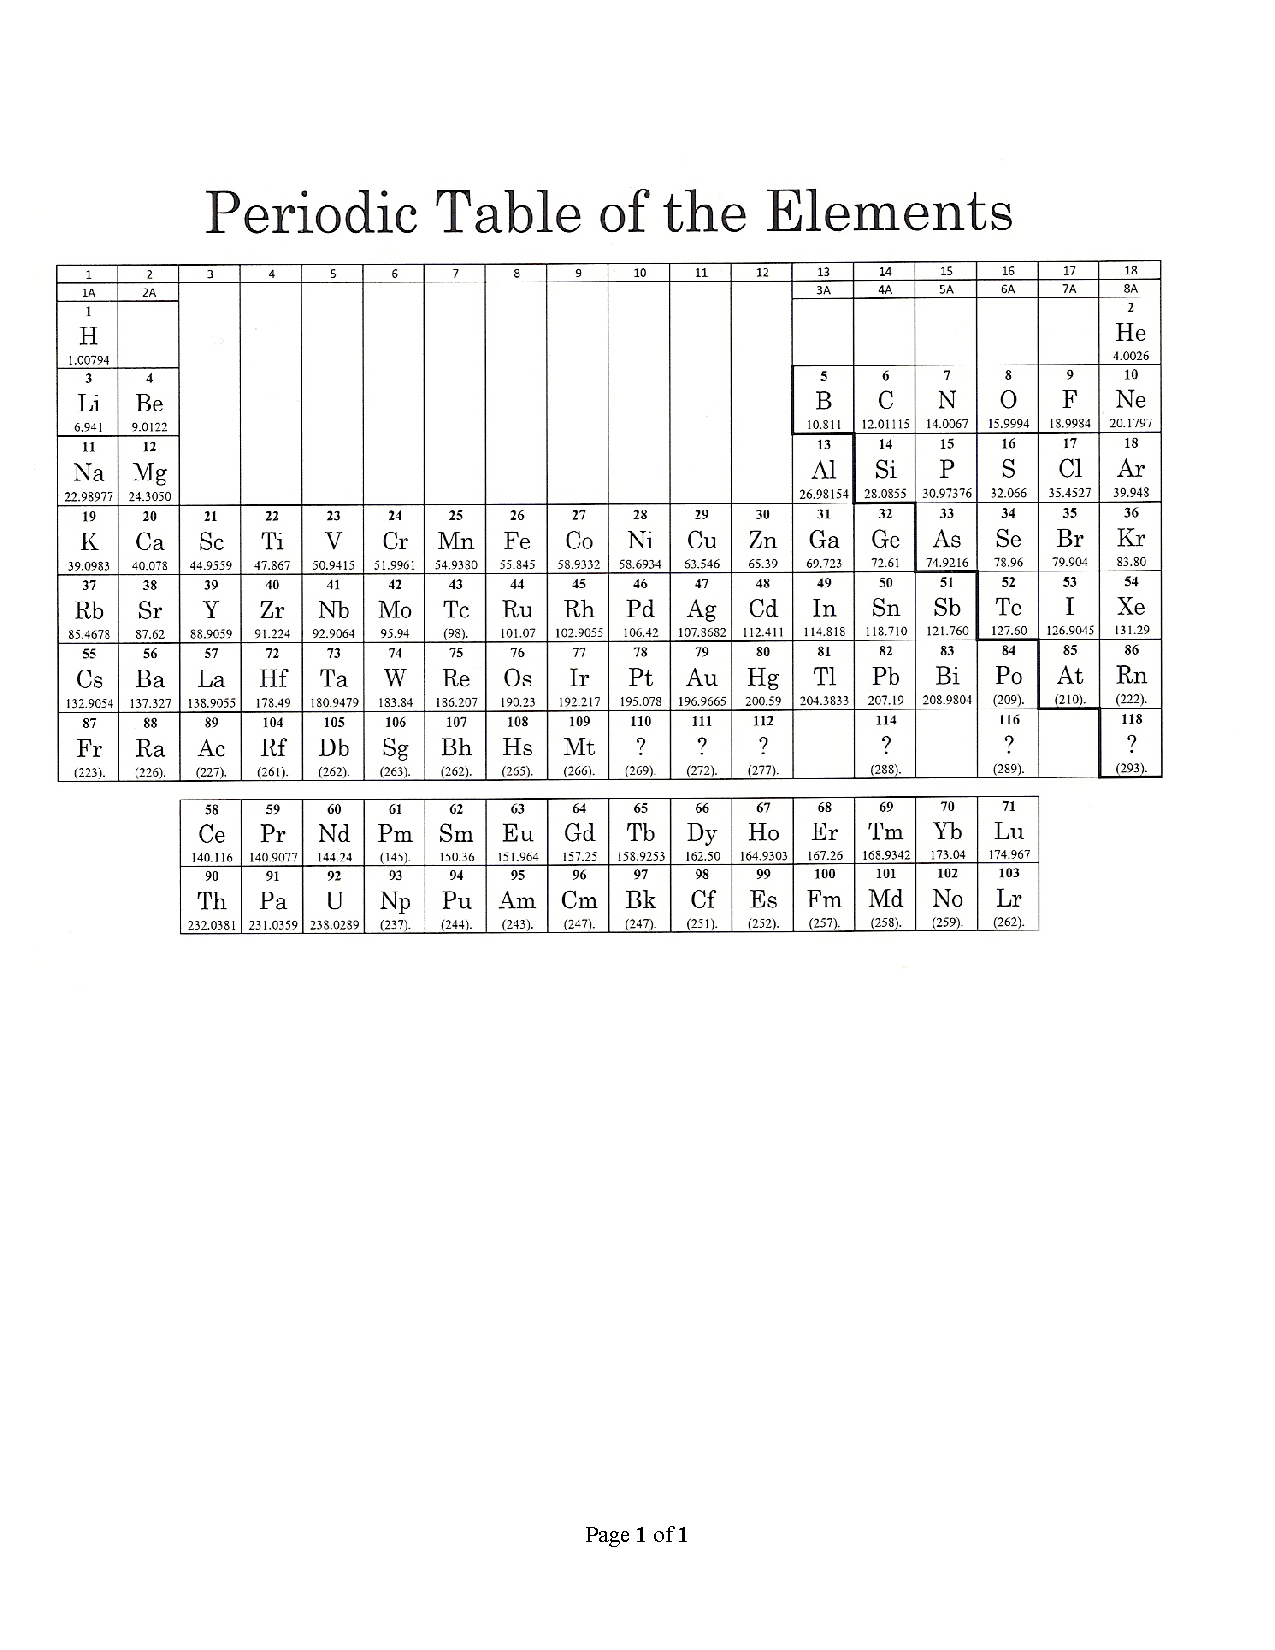
\includepdf[pages={-}]{Periodic Table for testing.pdf}

\end{document}